\chapter{Blide}

\textsf{
In questo capitolo viene presentato \emph{Blide} (Blite Integrated Development
Environment) un tool che racchiude un ambiente di esecuzione locale e
fornisce un intrefaccia grafica che permette di svolgere in maniera integrata
tutte le operazioni legate allo sviluppo di programmi Blite. Nella prima parte
del capitolo vengono descritte le caratteristiche e le funzionalità
dell'interfaccia, mentre nella seconda parte se ne presetano alcuni
esempi di utilizzo.
}

\section{Un IDE per Blite}

Oltre al motore di esecuzione si è realizzato un vero e proprio IDE per
sviluppare i programmi Blite. Questo strumento prevede la possibilità di
gestire i file con le definizioni dei processi, editarli, compilarli e metterli
in esecuzione. E' presente anche la funzionalità per visualizzare, tramite una
rappresentazione grafica, l'esecuzione delle istanze di processo.

Blide è stato realizzato tramite la piattaforma \emph{NetBeans Platform}
[NBPlatSite], un framework studiato per facilitare lo sviluppo di applicazioni
Java con interfaccia grafica. E' stato scelto tale progetto per la sua
completezza e per il modello architetturale offerto. 

NetBeans Platform permette allo sviluppatore di realizzare le proprie
applicazioni componendo diversi moduli, ciascuno dei quali offre una
funzionalità specifica. La modularizzazione molto fine e la gestione
formale delle dipendenze permettono di costruire applicazioni riuscendo a
selezionare in modo molto mirato solamente i moduli realmente necessari e
quindi a mantenere limitate le dimensioni complessive dell'applicazione. 

\begin{figure}[t!]
\begin{center}
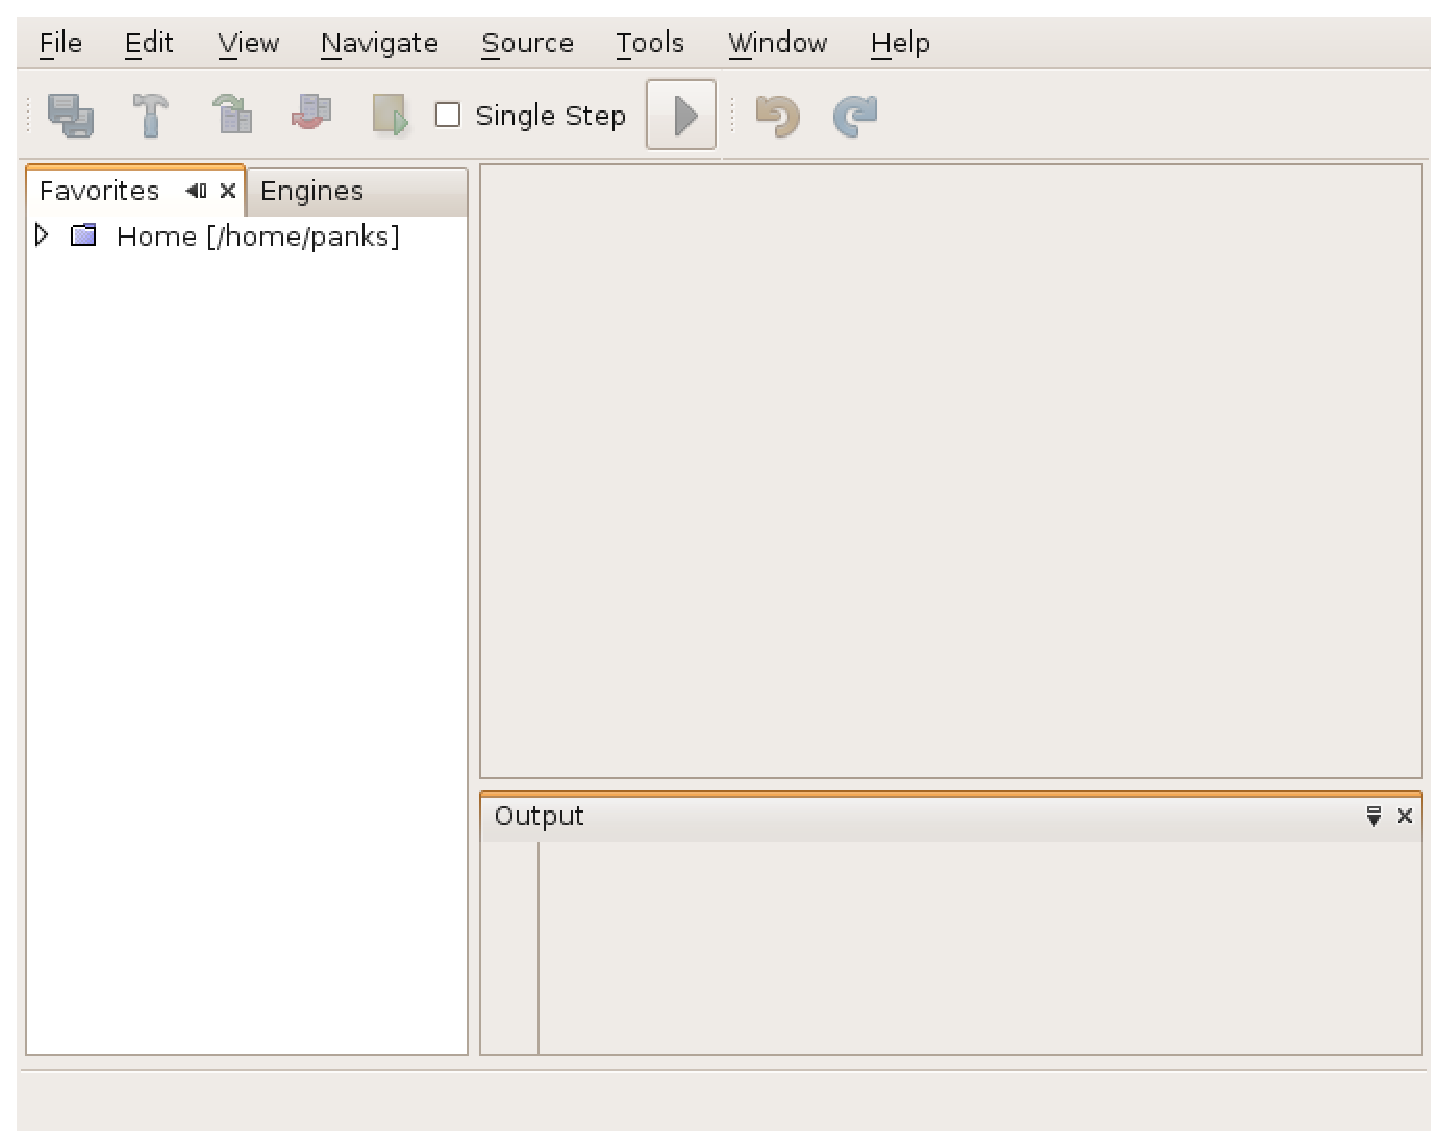
\includegraphics[scale=0.60]
{blide/dia/Blide1}
\caption[Blide Schermata]{Come si presenta Blide al primo avvio.}
  \label{fig:blide1}
\end{center}
\end{figure}
 
In Figura \ref{fig:blide1} è presentata l'interfaccia di Blide al primo avvio. 
Oltre alle consuete barre dei menù e dei pulsanti posizionate in alto
l'applicazione presenta quatro aree distinte

\begin{enumerate}
  \item Un pannello identificato dall'etichetta \emph{``Favorites''} che
  permette di accedere al filesystem e organizzare i file ``preferiti''
  in raggruppamenti logici.
  \item Un pannello identificato con l'etichetta \emph{``Engines''} in cui è
  possibile accedere ai motori di esecuzione attulamente disponibili, alle
  definizioni di processo e alle istanze create da queste.
  \item Un area centrale in cui verrano visualizzati gli editor con i file
  sorgenti e le raprresentazioni grafiche delle istanze esguite.
  \item Un pannello in basso in cui è possibile visualizzare l'output di
  sistema, come per esempio l'esito della compilazione dei programmi Blite.
\end{enumerate}

Di seguito andiamo ad analizzare più nel dettaglio queste aere funzionali
dell'interfaccia di Blide.

\subsubsection*{Favorites}

Abbiamo detto che questa area permette di accedere al filesystem, in realtà
non offre un'unica visone dell'albero come i consueti file manager, ma
permette in pratica di visualizzare direttamente più sotto alberi del
filesystem. Di fatto l'utente può selezionare un direcotry e con la funzione \emph{``Add to
Favoritess\ldots''} aggiungere tale direcory con tutto il suo sotto albero come
una nuova radice che compare direttamente nel pannello. In questo modo l'utente
si può creare una specie di \emph{Bookmarks} alle direttory a cui accede
maggiormente e in cui probabilemnte ha salvato i file di lavoro. Da notare che
tali configurazioni vengono salvate automaticamente dall'applicazione e al
successivo riavvio l'utente si troverà mantenute le scorciatoie alle directory
preferite. Al primo avvio l'applicazione mostrerà come unica risorsa favorita
la directory ``home'' dell'utente.

\begin{figure}[h]
\begin{center}
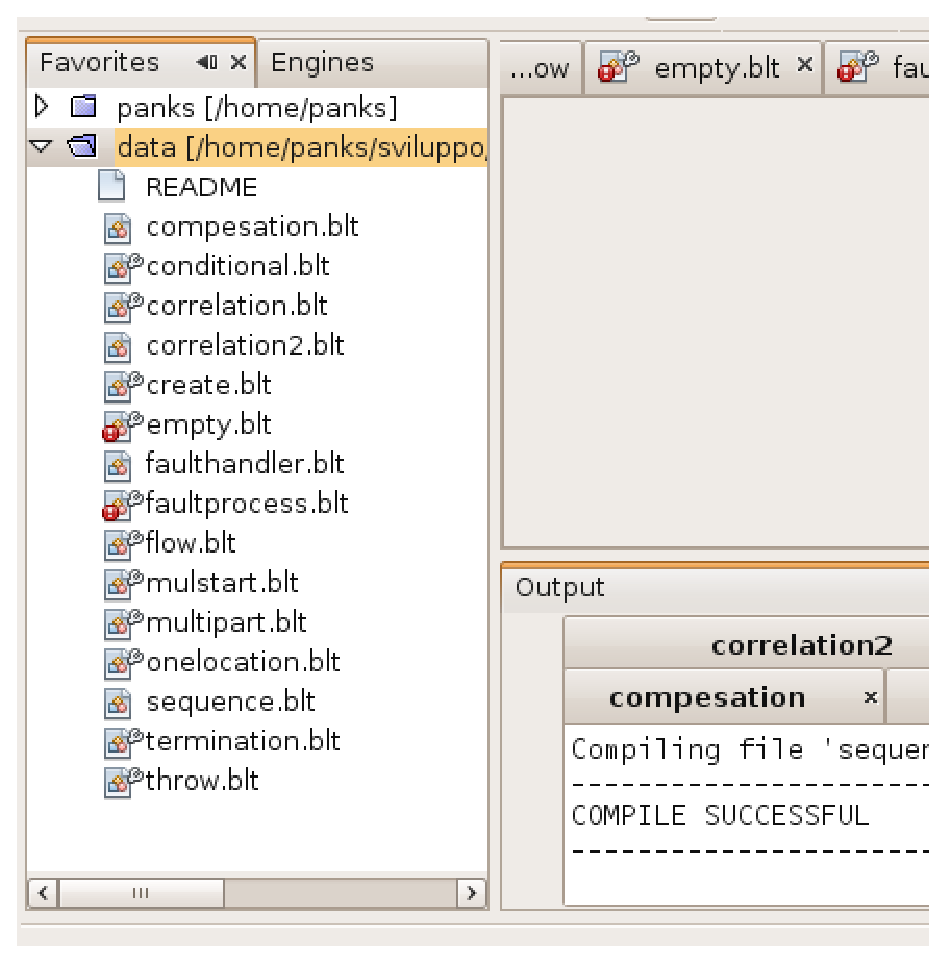
\includegraphics[scale=0.65]
{blide/dia/BlideFavo}
\caption[Il pannello ``Favorites'']{Una direcory con alcuni sorgenti Blite.}
  \label{fig:blideFavo}
\end{center}
\end{figure}

All'interno degli alberi di Favorites i file con estensione
\texttt{.blt} vengono riconosciuti come file sorgenti Blite e vengono
visualizzati con icone speciali. Inoltre l'applicazione decora tali icone in
base al fatto che i file necessito compilazione, siano stati compilati con successo o
presentino degli errori che ne hanno compromesso la compilazione. In Figura
\ref{fig:blideFavo} è rappresentato il pannello in cui è stato aggiunto la directory
\texttt{data} che contine una serie di file sorgenti Blite con le opportune
icone. In Tabella \ref{tab:bicons} sono rappresentate le varie icone associate ai
file Blite con il riferimento alla loro semantica.  
\\

\begin{table}
\begin{center}
\begin{tabular}{rp{0.7\textwidth}}

\includegraphics{blide/dia/biconto} & File Blite che deve essere compilato. Il
file non è mai stato compilato o ha subito modifiche dopo l'ultima
compilazione.\\ 
\includegraphics{blide/dia/biconko} & File Blite presenta errori di
compilazione. L'ultima compilazione eseguita sul file ha riportato errori.\\

\includegraphics{blide/dia/biconok} & File Blite compilato con successo.
Delle definizioni presenti nel file sono disponibili i modelli statici.\\
\end{tabular}
\caption{Icone associate ai file Blite con estensione \texttt{.blt}}
\label{tab:bicons}
\end{center}
\end{table}

Su ogni nodo rappresentante un file Blite possono essere eseguite diverse
azioni. In particolare tali azioni come è consuetudine nella applicazioni con
interfaccia grafica possono essere eseguite in modi diversi. 


